\documentclass[11pt,a4paper]{article}
\usepackage[spanish,es-nodecimaldot]{babel}	% Utilizar español
\usepackage[utf8]{inputenc}					% Caracteres UTF-8
\usepackage{graphicx}						% Imagenes
\usepackage[hidelinks]{hyperref}			% Poner enlaces sin marcarlos en rojo
\usepackage{fancyhdr}						% Modificar encabezados y pies de pagina
\usepackage{float}							% Insertar figuras
\usepackage[textwidth=390pt]{geometry}		% Anchura de la pagina
\usepackage[nottoc]{tocbibind}				% Referencias (no incluir num pagina indice en Indice)
\usepackage{enumitem}						% Permitir enumerate con distintos simbolos
\usepackage[T1]{fontenc}					% Usar textsc en sections
\usepackage{amsmath}						% Símbolos matemáticos
\usepackage{multirow}
\usepackage{mathtools}

% Comando para poner el nombre de la asignatura
\newcommand{\asignatura}{Arquitectura y Computación de Altas Prestaciones}
\newcommand{\autor}{Vladislav Nikolov Vasilev}
\newcommand{\titulo}{Práctica 3}
\newcommand{\subtitulo}{Paralelización del filtro de mediana}
\newcommand{\rama}{Ingeniería de Computadores}

% Configuracion de encabezados y pies de pagina
\pagestyle{fancy}
\lhead{\autor{}}
\rhead{\asignatura{}}
\lfoot{Grado en Ingeniería Informática}
\cfoot{}
\rfoot{\thepage}
\renewcommand{\headrulewidth}{0.4pt}		% Linea cabeza de pagina
\renewcommand{\footrulewidth}{0.4pt}		% Linea pie de pagina

\begin{document}
\pagenumbering{gobble}

% Pagina de titulo
\begin{titlepage}

\begin{minipage}{\textwidth}

\centering

%
\includegraphics[scale=0.5]{img/ugr.png}\\

\includegraphics[scale=0.3]{img/logo_ugr.jpg}\\[1cm]

\textsc{\Large \asignatura{}\\[0.2cm]}
\textsc{GRADO EN INGENIERÍA INFORMÁTICA}\\[1cm]

\noindent\rule[-1ex]{\textwidth}{1pt}\\[1.5ex]
\textsc{{\Huge \titulo\\[0.5ex]}}
\textsc{{\Large \subtitulo\\}}
\noindent\rule[-1ex]{\textwidth}{2pt}\\[3.5ex]

\end{minipage}

%\vspace{0.5cm}
\vspace{0.7cm}

\begin{minipage}{\textwidth}

\centering

\textbf{Autor}\\ {\autor{}}\\[2.5ex]
\textbf{Rama}\\ {\rama}\\[2.5ex]
\vspace{0.3cm}


\includegraphics[scale=0.3]{img/etsiit.jpeg}

\vspace{0.7cm}
\textsc{Escuela Técnica Superior de Ingenierías Informática y de Telecomunicación}\\
\vspace{1cm}
\textsc{Curso 2019-2020}
\end{minipage}
\end{titlepage}

\pagenumbering{arabic}
\tableofcontents
\thispagestyle{empty}				% No usar estilo en la pagina de indice

\newpage

\setlength{\parskip}{1em}

\newpage

\section{Introducción}

El objetivo de esta práctica es paralelizar, mediante \texttt{MPI}, un algoritmo secuencial que
trabaje con estructuras de datos 2D tales como podrían ser matrices. Una vez que se ha
paralelizado, se tienen que tomar medidas de los tiempos y obtener la ganancia según el número
de procesos que se utilice. Este estudio se tiene que hacer con dos problemas de tamaño
diferente, uno más pequeño y uno más grande.

\section{Algoritmo escogido: filtro de mediana}

El algoritmo que se ha escogido paralelizar es el \textbf{filtro de mediana}. Este es un
filtro bastante sencillo y utilizado en el procesamiento de imágenes ya que permite eliminar
el \textbf{ruido sal y pimienta} de estas. Este tipo de ruido se caracteriza por la presencia
de píxeles blancos y negros en la toda la imagen, los cuáles son producto de alguna perturbación
de la señal de la imagen. Un ejemplo se puede ver a continuación:

\begin{figure}[H]
    \centering
    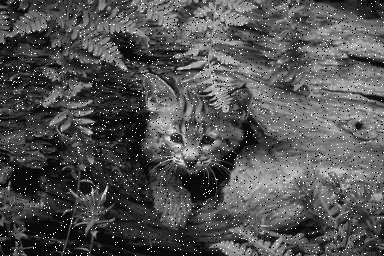
\includegraphics[scale=0.6]{img/cat.png}
    \caption{Imagen con ruido sal y pimienta.}
    \label{fig:cat}
\end{figure}

El algoritmo consiste en iterar sobre los píxeles de la imagen, coger una región de tamaño
$k \times k$ píxeles alrededor del actual (donde $k$ es el tamaño del filtro), ordenar
los valores y escoger el valor mediano, el cuál será el píxel de salida. Un ejemplo de este
procedimiento se puede ver a continuación:

\begin{figure}[H]
  \centering
  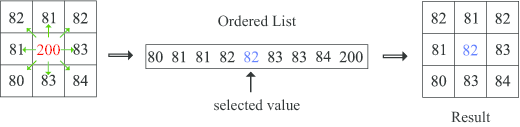
\includegraphics[scale=0.4]{img/median-filter.png}
  \caption{Ejemplo del filtro de mediana.}
  \label{fig:median-filter}
\end{figure}

Si aplicamos este filtro a la figura \ref{fig:cat}, obtendríamos el siguiente resultado:

\begin{figure}[H]
  \centering
  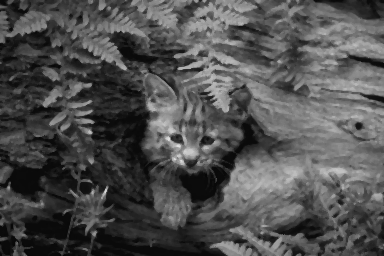
\includegraphics[scale=0.6]{img/filtered-cat}
  \caption{Imagen a la que se le ha aplicado el filtro de mediana.}
  \label{fig:filtered-cat}
\end{figure}

\section{Versión secuencial}

La versión secuencial del algoritmo se encuentra implementada en el archivo
\texttt{median-filter-sec.cpp}. No se va a discutir en demasiado detalle el algoritmo, ya que
se considera que la explicación anterior es suficiente, además de que en internet se puede
encontrar fácilmente una versión en pseudocódigo.

No obstante, sí que es importante destacar un detalle de la implementación. Calcular la mediana
en los bordes, en un principio, supondría adaptar el tamaño del filtro para que no se salga de
la imagen. Esto implicaría introducir bloques condicionales en el código, lo cuál
se traduce en comprobar en cada iteración que no se está intentando acceder a posiciones no
válidas de la imagen. Para evitar eso, se ha decidido replicar los bordes de la imagen, de manera
que se trabaja con una imagen más grande pero donde un filtro de tamaño $k \times k$ quepa
siempre. Esto a su vez implica, como es obvio, empezar a procear la imagen con un pequeño
desplazamiento, para que el filtro quepa exactamente. El resultado de salida es, obviamente,
una imagen del mismo tamaño que la original, eso no ha cambiado.

Esta replicación de los bordes se puede ver a continuación. Se ha utilizado un filtro
de tamaño 101 para que sea notable el resultado:

\begin{figure}[H]
  \centering
  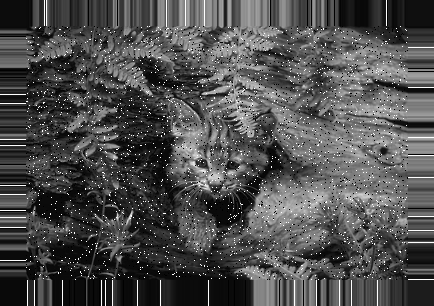
\includegraphics[scale=0.6]{img/borders-cat}
  \caption{Ejemplo de la replicación de bordes con filtro de tamaño $k = 101$.}
  \label{fig:borders-cat}
\end{figure}

\section{Paralelización}

La paralelización que se ha aplicado es parecida a la que se suele aplicar a la hora de
calcular un fractal de Mandelbrot con un programa paralelo.

Partiendo de una imagen de tamaño $w \times h$, donde $w$ es la anchura y $h$ la altura,
se determina que a cada proceso le corresponde un bloque de tamaño $w \times \frac{h}{n}$ píxeles
de la imagen original, donde $n$ es el número de procesos que se van a utilizar. Es importante
que $n$ sea un divisor de $h$, de forma que no queden filas sin asignar.

Una vez que se tiene la imagen con los bordes replicados, un proceso maestro envía el bloque con
los correspondientes bordes a los otros procesos, además de quedarse él con uno de ellos.
Adicionalmente, antes de enviar cada bloque, es necesario añadirle una parte del siguiente y/o
anterior bloque, lo cuál implicaría añadirle $\lfloor \frac{k}{2} \rfloor$ filas adicionales
de la imagen con los bordes replicados en caso de que solo se necesite información extra de un
bloque o $2 \cdot \lfloor \frac{k}{2} \rfloor$ en el caso de que se necesite la información de
dos bloques.

Esto se debe a que para aplicar el filtro en la primera y/o última
fila de cada bloque de la imagen original se necesita la información de las filas
contiguas, las cuáles están en el bloque anterior/siguiente. El hecho de añadirlas al bloque
que se va a enviar tiene una \textbf{ventaja} muy importante, y es que se evitan operaciones que
implican sincronización (envíos-recepciones), con lo cuál los tiempos de ejecución son menores.
Sin embargo, también tiene una \textbf{desventaja} bastante importante, y es que se necesita
memoria adicional para almacenar esas filas extra. Si el tamaño del filtro que se utiliza es muy
grande, esto implica enviar muchas filas extra, lo cuál se traduce en un mayor consumo de memoria.

Cada proceso, una vez que recibe su bloque, realiza los cálculos. Finalmente, el proceso maestro
recibe los datos del resto de procesos y crea la imagen final, donde obviamente también está el
resultado que ha producido dicho proceso.

El código donde está implementado todo esto se puede encontrar en el fichero
\texttt{median-filter.cpp}.

\section{Experimentación realizada}

Tal y como se ha dicho al principio, se ha experimentado con dos problemas de distinto tamaño,
o lo que viene a ser lo mismo, se han utilizado dos imágenes de distinto tamaño, y se han tomado
las medidas de tiempo pertinentes.

Ambas imágenes están y blanco y negro, con lo cuál se puede utilizar un solo canal
a la hora de aplicar el filtro. La primera de ellas es una imagen de un búho que tiene
un tamaño de $1024 \times 512$ píxeles, y se encuentra en el archivo \texttt{noisy-owl.jpg}.
La segunda es una imagen de una ilusión óptica, la cuál tiene un tamaño de $8192 \times 4096$
píxeles, y se encuentra en el archivo \texttt{noisy-illusion.jpg}.

Se han realizado pruebas con 1, 2 y 4 procesos, ya que es un número de procesos que es divisor
de las alturas de las imágenes utilizadas, además de que en la máquina local de la que se
dispone se pueden ejecutar, como mucho, 6 procesos. Cada ejecución se ha repetido tres
veces y se han anotado los resultados. De los resultados obtenidos para cada caso se escogerá
aquel que tenga un menor tiempo de ejecución total. Esto se hará para cada uno de los problemas.
Luego, con los resultados obtenidos, se calculará la ganancia y se hará un estudio de esta.

Es importante destacar que en todos los casos se ha utilizado un filtro de tamaño $k = 7$, ya
que anteriormente se han hecho pruebas y se ha visto que con un filtro de ese tamaño los
resultados obtenidos son buenos.

\section{Resultados en la máquina local}

En las siguientes tablas se pueden ver los resultados obtenidos para el problema pequeño
y el grande en la máquina local, destacando los mejores en negrita:

\begin{table}[H]
\centering
\begin{tabular}{|c|c|c|c|c|}
\hline
\textbf{Núm. procesos} & \textbf{T. inicialización} & \textbf{T. cómputo} & \textbf{T. recepción} & \textbf{T. total} \\ \hline
\multirow{3}{*}{\textbf{\begin{tabular}[c]{@{}c@{}}1\\ proceso\end{tabular}}} & 0.283196 & 0.464572 & 0.000259541 & 0.748028 \\ \cline{2-5} 
 & 0.285312 & 0.466776 & 0.000257954 & 0.752346 \\ \cline{2-5} 
 & \textbf{0.250298} & \textbf{0.482575} & \textbf{0.000265891} & \textbf{0.733139} \\ \hline
\multirow{3}{*}{\textbf{\begin{tabular}[c]{@{}c@{}}2\\ procesos\end{tabular}}} & 0.282476 & 0.238545 & 0.00132745 & 0.522349 \\ \cline{2-5} 
 & 0.293897 & 0.236872 & 0.00112881 & 0.531897 \\ \cline{2-5} 
 & \textbf{0.254151} & \textbf{0.236905} & \textbf{0.000592914} & \textbf{0.49165} \\ \hline
\multirow{3}{*}{\textbf{\begin{tabular}[c]{@{}c@{}}4\\ procesos\end{tabular}}} & 0.275051 & 0.128427 & 0.000937591 & 0.404415 \\ \cline{2-5} 
 & \textbf{0.26996} & \textbf{0.12312} & \textbf{0.00112293} & \textbf{0.394203} \\ \cline{2-5} 
 & 0.285471 & 0.124165 & 0.00120879 & 0.410844 \\ \hline
\end{tabular}
\caption{Tiempos obtenidos en la máquina local para el problema pequeño.}
\label{tab:local-small}
\end{table}

\begin{table}[H]
\centering
\begin{tabular}{|c|c|c|c|c|}
\hline
\textbf{Núm. procesos} & \textbf{T. inicialización} & \textbf{T. cómputo} & \textbf{T. recepción} & \textbf{T. total} \\ \hline
\multirow{3}{*}{\textbf{\begin{tabular}[c]{@{}c@{}}1\\ proceso\end{tabular}}} & \textbf{1.62949} & \textbf{25.2294} & \textbf{0.018211} & \textbf{26.8771} \\ \cline{2-5} 
 & 1.57688 & 25.3627 & 0.0183813 & 26.958 \\ \cline{2-5} 
 & 1.61837 & 26.0702 & 0.0197927 & 27.7084 \\ \hline
\multirow{3}{*}{\textbf{\begin{tabular}[c]{@{}c@{}}2\\ procesos\end{tabular}}} & \textbf{1.60864} & \textbf{13.9969} & \textbf{0.0131912} & \textbf{15.6187} \\ \cline{2-5} 
 & 1.74574 & 15.4248 & 0.0146795 & 17.1852 \\ \cline{2-5} 
 & 1.7108 & 15.0814 & 0.0136675 & 16.8058 \\ \hline
\multirow{3}{*}{\textbf{\begin{tabular}[c]{@{}c@{}}4\\ procesos\end{tabular}}} & \textbf{1.6241} & \textbf{7.57243} & \textbf{0.0109807} & \textbf{9.20751} \\ \cline{2-5} 
 & 1.67817 & 7.85654 & 0.0114578 & 9.54617 \\ \cline{2-5} 
 & 1.67679 & 7.81392 & 0.011557 & 9.50227 \\ \hline
\end{tabular}
\caption{Tiempos obtenidos en la máquina local para el problema grande.}
\label{tab:local-big}
\end{table}

Vemos que, para el problema pequeño, el tiempo de inicialización se mantiene más o menos
constante, mientrsa que el de cómputo se va reduciendo y el de recepción va aumentando.
Este comportamiento es el esperado, ya que hay demasiados pocos procesos para que se note
demasiado la inicialización, y al aumentar dicho número, el tiempo de cómputo va a disminuir
y el de recepción va a aumentar, ya que hay que esperar que más procesos se sincronicen con
el maestro que recibe los datos.

En cuanto al problema grande, vemos que el comportamiento de los tiempos es el mismo
en cuanto al tiempo de inicialización y de cómputo, mientras que el de recepción va disminuyendo
poco a poco. Esto se puede deber a que, al ir aumentando el número de procesos, la cantidad
de datos que tiene que enviar cada uno es menor, y por tanto, el tiempo va disminuyendo.
Posiblemente, si seguimos aumentando el número de procesos, el tiempo de recepción puede
que disminuya algo más, pero habrá un momento en el que, si hay demasiados procesos, se llegue
a producir un \textit{overhead} por la comunicación introducida.

La evolución de los tiempos de ejecución en función del número de procesos se puede ver
en la siguiente gráfica, la cuál está representada en escala logarítimica:

\begin{figure}[H]
  \centering
  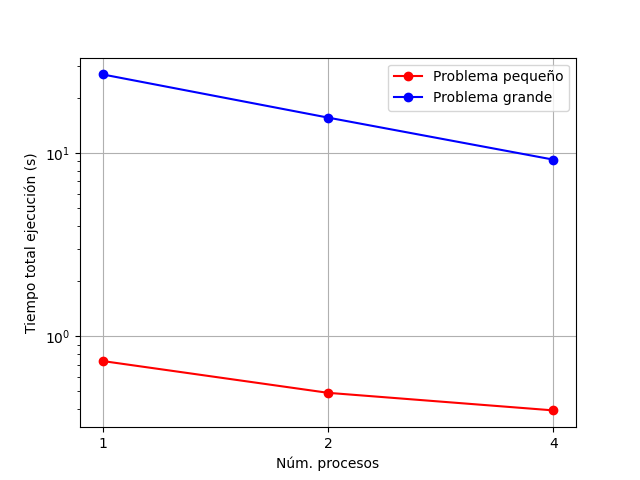
\includegraphics[scale=0.6]{img/local-tiempos}
  \caption{Evolución de los tiempos de ejecución en función del número de procesadores para
  los dos problemas en la máquina local.}
  \label{fig:local-tiempos}
\end{figure}

Tal y como se podía ver en las tablas \ref{tab:local-small} y \ref{tab:local-big}, los tiempos
totales van decreciendo, lo cuál es un comportamiento esperado al introducir más procesos.

Una vez que hemos estudiado los tiempos, vamos a ver las ganancias. En la siguiente tabla
y gráfica se pueden ver los resultados obtenidos:

\begin{table}[H]
\centering
\begin{tabular}{|c|c|c|}
\hline
\textbf{Núm. procesos} & \textbf{\begin{tabular}[c]{@{}c@{}}Ganancia\\ problema pequeño\end{tabular}} & \textbf{\begin{tabular}[c]{@{}c@{}}Ganancia\\ problema grande\end{tabular}} \\ \hline
1 & 1 & 1 \\ \hline
2 & 1.49118072 & 1.72082824 \\ \hline
4 & 1.85980066 & 2.91904109 \\ \hline
\end{tabular}
\caption{Ganancia para los problemas pequeño y grande en la máquina local según el número de procesos.}
\label{tab:speed-local}
\end{table}

\begin{figure}[H]
  \centering
  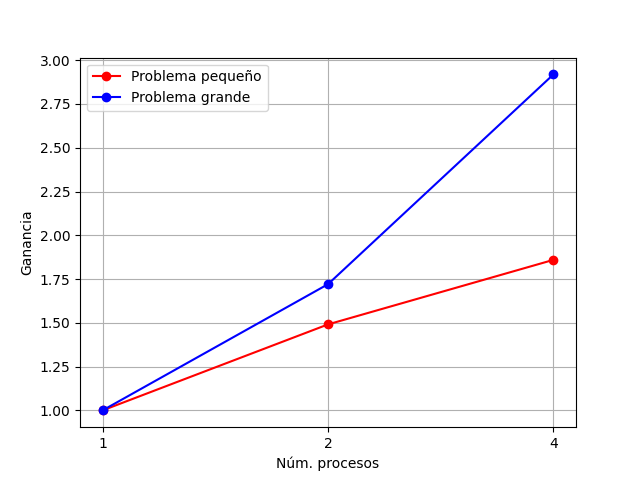
\includegraphics[scale=0.6]{img/local-ganancia}
  \caption{Evolución de la ganancia según el número de procesos para los dos problemas en
  la máquina local.}
  \label{fig:local-ganancia}
\end{figure}

Viendo los resultados podemos decir que, en este caso, la ganancia obtenida en el
problema pequeño es mucho menor que la obtenida en el problema grande. Esto se debe
a que al ir aumentando el número de procesos, el tiempo de ejecución del problema grande
ha ido disminuyendo de manera mucho más notable que el del problema pequeño. Por tanto,
la ganancia en el caso del problema grande va a ser bastante mayor que la del pequeño.
De aquí podríamos concluir que a lo mejor, en la máquina local, para problemas pequeños
no merece mucho la pena paralelizar, si no que lo mejor sería hacerlo con problemas
más grandes.

Otra cosa que se podría decir es que ambas ganancias son sublineal, ya que en todos los casos
la ganancia está por debajo del número de procesos utilizados (excepto claro está en el
caso de un solo proceso). Por tanto, podríamos decir que la ganancia está acotada y que
llegará un momento en el que, por muchos procesos que se utilicen, el tiempo de ejecución
no mejoraría, si no que de hecho, podría empezar a empeorar debido al \textit{overhead}.
A pesar de que ambas ganancias son sublineales, parece que la ganancia del problema
pequeño se va a estancar bastante antes que la del grande, el cuál parece que sigue mejorando
según más procesos se vayan utilizando, aunque como hemos dicho anteriormente, también
llegará un punto en el que se estanque. No obstante, el número de procesos con el que
va a suceder esto va a ser bastante mayor que el del pequeño, el cuál parece que ya
está llegando a su límite.

\section{Resultados en \texttt{atcgrid}}

En las siguientes tablas se pueden ver los resultados obtenidos para el problema pequeño
y el grande en \texttt{atcgrid}, destacando de nuevo los mejores en negrita:

\begin{table}[H]
\centering
\begin{tabular}{|c|c|c|c|c|}
\hline
\textbf{Núm. procesos} & \textbf{T. inicialización} & \textbf{T. cómputo} & \textbf{T. recepción} & \textbf{T. total} \\ \hline
\multirow{3}{*}{\textbf{\begin{tabular}[c]{@{}c@{}}1\\ proceso\end{tabular}}} & 0.0361632 & 1.08516 & 0.000683753 & 1.122 \\ \cline{2-5} 
 & 0.0360606 & 1.13961 & 0.000684055 & 1.17635 \\ \cline{2-5} 
 & \textbf{0.032494} & \textbf{1.06818} & \textbf{0.000696268} & \textbf{1.10137} \\ \hline
\multirow{3}{*}{\textbf{\begin{tabular}[c]{@{}c@{}}2\\ procesos\end{tabular}}} & 0.0472678 & 0.532573 & 0.0199399 & 0.599781 \\ \cline{2-5} 
 & \textbf{0.0493438} & \textbf{0.53841} & \textbf{0.00731511} & \textbf{0.595069} \\ \cline{2-5} 
 & 0.0378574 & 0.553381 & 0.00450031 & 0.595739 \\ \hline
\multirow{3}{*}{\textbf{\begin{tabular}[c]{@{}c@{}}4\\ procesos\end{tabular}}} & 0.0537713 & 0.284362 & 0.0072266 & 0.34536 \\ \cline{2-5} 
 & 0.0503169 & 0.267138 & 0.0264396 & 0.343895 \\ \cline{2-5} 
 & \textbf{0.0417321} & \textbf{0.277327} & \textbf{0.00722497} & \textbf{0.326284} \\ \hline
\end{tabular}
\caption{Tiempos obtenidos en \texttt{atcgrid} para el problema pequeño.}
\label{tab:atc-small}
\end{table}

\begin{table}[H]
\centering
\begin{tabular}{|c|c|c|c|c|}
\hline
\textbf{Núm. procesos} & \textbf{T. inicialización} & \textbf{T. cómputo} & \textbf{T. recepción} & \textbf{T. total} \\ \hline
\multirow{3}{*}{\textbf{\begin{tabular}[c]{@{}c@{}}1\\ proceso\end{tabular}}} & 1.1827 & 51.9295 & 0.031004 & 53.1432 \\ \cline{2-5} 
 & 1.16487 & 53.4686 & 0.0310805 & 54.6646 \\ \cline{2-5} 
 & \textbf{1.16376} & \textbf{51.4565} & \textbf{0.0310337} & \textbf{52.6512} \\ \hline
\multirow{3}{*}{\textbf{\begin{tabular}[c]{@{}c@{}}2\\ procesos\end{tabular}}} & 1.30696 & 27.5587 & 0.169182 & 29.0348 \\ \cline{2-5} 
 & 1.30225 & 27.7085 & 0.158999 & 29.1698 \\ \cline{2-5} 
 & \textbf{1.31272} & \textbf{27.4243} & \textbf{0.16786} & \textbf{28.9049} \\ \hline
\multirow{3}{*}{\textbf{\begin{tabular}[c]{@{}c@{}}4\\ procesos\end{tabular}}} & 1.33152 & 14.2947 & 0.160236 & 15.7865 \\ \cline{2-5} 
 & \textbf{1.32545} & \textbf{14.2123} & \textbf{0.161904} & \textbf{15.6996} \\ \cline{2-5} 
 & 1.30741 & 14.3261 & 0.172918 & 15.8064 \\ \hline
\end{tabular}
\caption{Tiempos obtenidos en \texttt{atcgrid} para el problema grande.}
\label{tab:atc-big}
\end{table}

Si estudiamos los resultados, vemos que en ambos casos los tiempos totales van disminuyendo
a medida que se aumentan el número de procesos utilizados. Vemos que en ambos casos el tiempo
de cómputo va disminuyendo según el número de procesos utilizados, además de que los tiempos
de inicialización y recepción aumentan al pasar de un proceso a dos y luego se mantienen más o
menos iguales. Esto puede deberse a que ahora los datos sí que viajan por la tarjeta de red
hasta llegar a los otros nodos, a diferencia de lo que sucede en la máquina local, donde
van hasta la tarjeta de red y vuelven, sin enviarse.

A diferencia de los resultados obtenidos en la máquina local vemos que aquí, en general, los
tiempos son algo más grandes (menos los de inicialización que son más pequeños). Por una parte,
el hecho de que los tiempos sean en general mayores puede deberse a que el procesador de la
máquina local sea bastante más potente que el de \texttt{atcgrid}, ya que posiblemente sea capaz
de ejecutar un mayor número de instrucciones por segundo que el del servidor al tener el
primero una frecuencia mayor. Por otra parte, el hecho de que los tiempos de inicialización
sean menores puede significar que los procesadores de los nodos de un servidor están más
preparados para ejecutar código de este tipo, ya que es algo que se supone que tienen que hacer
frecuentemente, por lo tanto se espera que dicho tiempo sea lo más pequeño posible.

A continuación podemos ver una gráfica con la evolución de los tiempos de ejecución en función
del número de procesos:

\begin{figure}[H]
  \centering
  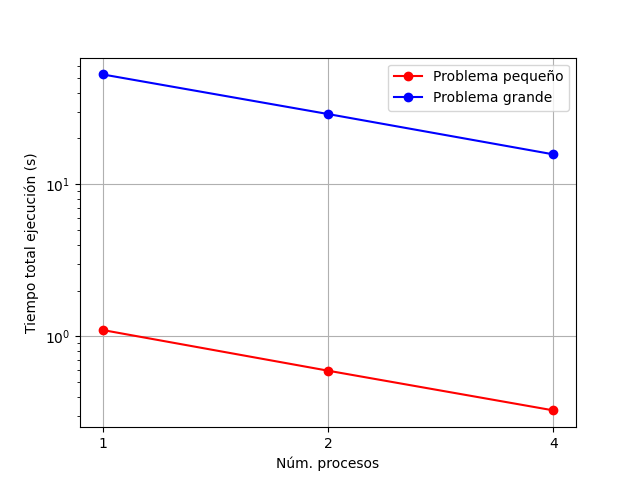
\includegraphics[scale=0.6]{img/atcgrid-tiempos}
  \caption{Evolución de los tiempos de ejecución en función del número de procesadores para
  los dos problemas en \texttt{atcgrid}.}
  \label{fig:atcgrid-tiempos}
\end{figure}

Podemos ver que, al igual que antes, los tiempos van decreciendo cuantos más procesos se
utilicen. No obstante, las dos rectas que representan la evolución parece que son paralelas aquí,
a diferencia de lo que sucedía en elcaso anterior, donde la recta del problema pequeño
sufría una pequeña curvatura.

Una vez que hemos analizado los tiempos, vamos a estudiar la ganancia. A continuación se
ofrece una tabla junto con su correspondiente gráfica:

\begin{table}[H]
\centering
\begin{tabular}{|c|c|c|}
\hline
\textbf{Núm. procesos} & \textbf{\begin{tabular}[c]{@{}c@{}}Ganancia\\ problema pequeño\end{tabular}} & \textbf{\begin{tabular}[c]{@{}c@{}}Ganancia\\ problema grande\end{tabular}} \\ \hline
1 & 1 & 1 \\ \hline
2 & 1.85082738 & 1.82153199 \\ \hline
4 & 3.37549497 & 3.35366506 \\ \hline
\end{tabular}
\caption{Ganancia para los problemas pequeño y grande en \texttt{atcgrid} según el número de procesos.}
\label{tab:speed-atcgrid}
\end{table}

\begin{figure}[H]
  \centering
  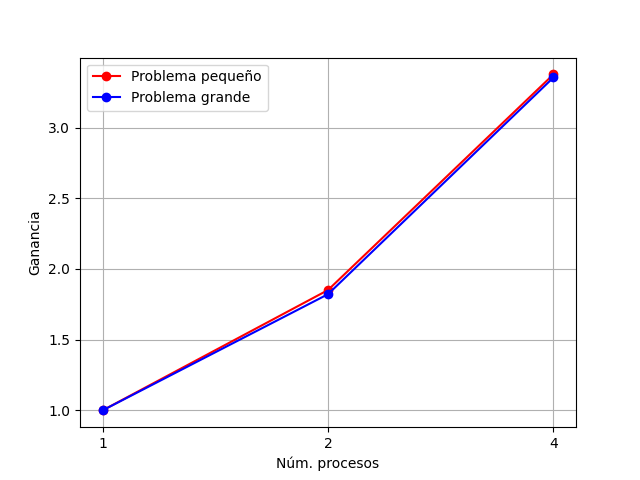
\includegraphics[scale=0.6]{img/atcgrid-ganancia}
  \caption{Evolución de la ganancia según el número de procesos para los dos problemas en
  \texttt{atcgrid}.}
  \label{fig:atcgrid-ganancia}
\end{figure}

En este caso podemos observar que, a pesar de que los tiempos de ejecución han sido peores, la
ganancia obtenida es mucho mayor, sobre todo en el caso del problema pequeño, donde si
la comparamos con la figura \ref{fig:local-ganancia}, vemos que ha habido muchísima mejora,
superando la barrera del 2 en la que parecía que se estancaba en dicho ccaso.

Las ganancias obtenidas para los dos problemas son bastante similares y van aumentando
casi a la par. Esto nos indica que, a diferencia del caso anterior, aquí merece la pena
paralelizar independientemente del tamaño del problema, ya que obtendremos unos mejores
tiempos al utilizar más procesos. No obstante, tal y como pasó anteriormente, ambas
ganancias son sublineales, con lo cuál la ganancia máxima que se puede obtener está acotada.
Esto significa que llegará un momento en el que aumentar el número de procesos no va a implicar
una mejora, y puede que incluso los tiempos empiecen a empeorar, tal y como se ha explicado antes.
Sin embargo, en este caso parece que el límite es mayor que en el caso de la máquina local,
con lo cuál se podrían utilizar un mayor número de procesos antes de llegar a ese tope.

\section{Conclusiones}

Después de este pequeño estudio, podemos concluir una serie de cosas. Por una parte, los
servidores permiten obtener una mayor escalabildad ejecutando código paralelo que los equipos
de sobremesa/portátiles. Además, si se tiene una configuración fácilmente expandible (es decir,
que sea fácil añadir más nodos de cómputo), la escalabilidad puede ser mucho mayor incluso.
Por otra parte, tal y como hemos visto en el caso de la máquina local con el problema pequeño,
tenemos que plantearnos si, por el tamaño del problema, merece la pena paralelizar el código,
ya que podría darse el caso de que la ganancia obtenida al paralelizar es demasiado pequeña
y no merece la pena el esfuerzo debido a que siempre se trabaja con problemas pequeños.

En resumen, hemos visto la importancia de paralelizar código para problemas grandes, que se puede
estudiar si merece la pena paralelizar para problemas pequeños dependiendo del tipo de
arquitectura para el que se usará el programa, y que los servidores tienen una mayor escalabilidad
que los equipos de gama baja.

\end{document}

